% !TEX root = ../my-thesis.tex
%
\chapter{Conclusions and Future Perspectives}
\label{sec:conclusion}

\cleanchapterquote{Arandu ndaha'\'ei mba'e ojejogu\'ava, ha'e katu yvyra ra'yi o\~ne\~notyva ha okaku\'aava \~nandepype.}{Paraguayan Proverb}{}

\section{Summary of Contributions}
This work was motivated by the need to develop robust and efficient methodologies for \gls{uq} in the presence of model mis-specification and discontinuous responses. These research axes are particularly relevant for the field of in-flight icing research, where the models used to simulate the physical phenomena are flawed and the response surfaces of interest are often discontinuous. In this section, we are going to recap the different research questions that inspired this manuscript, analyze their motivation, summarize how they were answered by this manuscript, and highlight the main limitations and what can be done to further improve the state-of-the-art of \gls{uq}.

\subsection{Part I}

A detailed analysis of the state-of-the-art techniques identified a critical gap in the way the model error is treated in the calibration process. Most of the existing techniques dismiss a \gls{fb} framework, in which both the model and model error are learned simultaneously from the available data, in favor of a modular framework, in which the model error is learned first and then used to calibrate the model. While this approach is computationally more efficient, it is inferior to the \gls{fb} framework, as the latter provides a more accurate representation of the uncertainty in the parameters of interest, by allowing the model error to inform the model parameters and vice versa. 

\smallskip
From this critical gap the first research question of this thesis emerged: how to develop a modular calibration framework that can provide a more accurate representation of the uncertainty in the parameters of interest, without increasing the dimensionality of the calibration problem? This question was addressed in Part I of this thesis, which focused on the development of a novel calibration framework, the \gls{cmp} method, which is a modular framework that can provide a more accurate representation of the uncertainty in the parameters of interest, without increasing the dimensionality of the calibration problem. The \gls{cmp} method is based on the idea of learning a deterministic function that maps the parameters of interest to the model error hyperparameters, which is often more flexible than a standard modular approach. Under very mild assumptions (that were shown to be less strict than the ones of a Laplace approximation), we were able to show that the \gls{cmp} method is equivalent to the \gls{fb} framework.

\smallskip
The introduction of a functional mapping between parameters and hyperparameters opened the door to a second research question: how to efficiently query this functional mapping, which is often expensive to evaluate? This question was addressed in Chapter~\ref{sec:surr}, where we developed a surrogate-based acceleration technique that can be used to efficiently query the functional mapping, which is particularly useful to make the \gls{cmp} method computationally feasible for real-world applications. We developed an ad-hoc sampling strategy that builds the training set in an iterative way. This ensures that the growth of the training set is controlled, and that it addresses regions in which the surrogate mapping is both uncertain and relevant for the calibration process. 

\smallskip
Finally, in Chapter~\ref{sec:cfd} we presented an application to various calibration strategies (including \gls{cmp}) to a problem in hypersonic flow. The field of hypersonic flows shares similar technical and methodological challenges with aircraft icing. In particular, experimental tests are expensive and limited to a few \glspl{qoi} and computational models are often mis-specified. A fruitful collaboration with the \gls{vki} allowed us to develop a framework to calibrate the chemical properties of \glspl{tpm} using few experimental data and mis-specified models. Through a series of synthetic test cases, we have demonstrated that calibration with model error can be used to characterize these \glspl{tpm}.

\smallskip
The main limitation of this chapter is the lack of high-dimensional test cases. Although most real-world engineering problems do not require millions of parameters or experimental data points~\cite{uq_theory} (in contrast with some other \gls{ml} applications~\cite{gp_rasmussen}), the first part of this thesis leverages test cases with a maximum of $10$ parameters and hyperparameters and $15$ experimental data points. The \textit{curse of dimensionality} teaches that methods that we assume to be working well in moderate dimensions require a completely different treatment in higher dimensions, and assumptions that we deem reasonable in low dimensions may completely fail in higher ones. For this reason, a critical investigation that compares the true computational cost and precision of \gls{fb}, modular and \gls{cmp}-like methods in high dimensional parameter spaces is required. Furthermore, dealing with high-dimensional experimental datasets may require the use of different techniques, whose compatibility with the proposed approaches needs to be analyzed.

\smallskip
On a more methodological side, when creating a surrogate model for the model error hyperparameters, we did not include the construction of the surrogate model of the computer code in the loop. Although the motivations given were reasonable, building a surrogate model of the computer code in an adaptive way has some benefits on the order of convergence, and is standard practice in the current research paradigms, see~\cite{lucor2018, phd3} for some examples. Investigating strategies to build both surrogate models simultaneously would further strengthen the methodological aspects of \gls{as} strategies.

\smallskip
Finally, concerning the work on the characterization of the chemical properties of \gls{tpm} materials, one should first investigate \textit{where} and \textit{how many} experimental points to place. In the results, we showed how the posterior changes with respect to the size of the experimental dataset but did not consider how to increase it. In Chapter~\ref{sec:surr} we presented a way to robustly increase the size of the \gls{ndoe}. Treating the \gls{doe} and \gls{ndoe} differently is not justified and one should investigate whether adaptive techniques can be leveraged to build the \gls{doe} more effectively. The biggest challenge in hypersonic flows is the lack of rich datasets, and it is not uncommon to be limited to fewer than 10 experiments. 


\subsection{Part II}

The development of the second part of this manuscript stemmed from the need to develop a surrogate strategy compatible with non-smooth responses. Indeed, surrogate models are the backbone of the vast majority of \gls{uq} methodologies, since they replace calls to expensive computer codes. Discontinuities in the response surface or its gradients pose a significant challenge for surrogate modeling, as the vast majority of surrogate modeling techniques assume smoothness in the response surface. 

\smallskip
In particular, \glspl{gp} with stationary covariance functions, although capable of interpolating discontinuous data, may produce oscillations or be challenging to train, with their hyperparameters often converging to biased values. Similarly, \glspl{pce} either produce a massive error everywhere in the domain or produce spurious oscillations. The current state-of-the-art mentions a plethora of problem (domain) specific approaches that practitioners use to know in advance where the discontinuity may be and, consequently, how to treat it. Such approaches are not desirable as they are hard to generalize to different settings. Many problem-independent approaches are also present, but they either consider very simple shapes for the discontinuities or rely on complex sampling algorithms. When investigating the state-of-the-art, we were particularly inspired by a recent technique, proposed by~\cite{Sudret2023}, that uses a combination of 3 common \gls{ml} techniques (clustering, classification and regression) to localize the discontinuity and build a robust surrogate model. Their technique is limited by the fact that these 3 techniques are applied independently, often resulting in a poor surrogate model.

\smallskip
In this regard, the last research question that this thesis addresses is how to build a surrogate model for a discontinuous function, without relying on expert or prior knowledge. 

\smallskip
The answer to this question is found in Chapter~\ref{sec:clustering}, in which we develop an algorithm to build a piecewise-continuous surrogate model. This form of surrogate model is very effective in modeling discontinuous responses and, by introducing some inter-model averaging, can be used to produce continuous and differentiable response surfaces. We were inspired by the approach in~\cite{Sudret2023}, and used the same classification and regression techniques. The main difference is that our approach is not static, but the classification and regression stages constantly inform the clustering one in an iterative fashion. We have shown that our approach can deal with a wide range of discontinuities or challenging behaviors across multiple dimensions and \gls{doe} sizes, even dealing with non-convex cluster shapes. Furthermore, introducing an iterative improvement improves upon the \gls{dp}-\gls{gmm} strategy of~\cite{Sudret2023}, without requiring complex sampling or optimization strategies.

\smallskip
The main limitation of the proposed approach lies in its initialization. In particular, our approach takes an initial clustering and iteratively improves it. Its results are therefore very dependent on the choice of such initial partition, a problem that is exacerbated by the fact that it is unable to enrich the partition by spawning new clusters. This is a problem for initial partitions that contain too few clusters, for which no sequence of moves can realistically produce a better one, and initial partitions that have too many clusters, for which the final clustering is able to identify the discontinuities but not the correct number of clusters. To tame both issues, we have introduced a stochastic optimization strategy that promises to better explore the search space. Although yielding promising results, we are not able to improve pathologically bad partitions and have to rely on an extra temperature hyperparameter. 

\smallskip
To overcome the over-clustering problem, we introduced a primitive strategy that merges clusters that mix. The success (or failure) of this strategy relies on having an optimal combination of two hyperparameters. Although it does not require careful fine-tuning, and we've shown that over-clustering is not necessarily a problem, such a strategy is not robust. One needs to investigate better merging strategies and strategies to enrich the partition.


\section{Future Perspectives}

This thesis opens up a series of possible methodological and applicative contributions in the field of \gls{uq} and surrogate modeling. Most of the research directions were already outlined in the previous sections, and concern the main limitations of this work. On the other hand, a very promising research direction comes from considering the union of Part I and Part II, which have been presented as disconnected research axes but are deeply connected. Indeed, as mentioned in the introduction, calibration requires the use of surrogate models to replace calls to the expensive computer code, and the surrogate model feeds upon precise knowledge of the possible value and distribution that its parameters can have. In other words, calibration informs the surrogate model on where it needs to be precise while surrogate models enable fast and efficient calibration. We have already seen this complex interplay in \S\ref{sec:surr}, in which we were able to construct a surrogate model that is precise in regions of the parameter space which are likely according to the calibration outcome.

\smallskip
So the question is, \textit{why not use an adaptive sampling strategy to build a piecewise surrogate model?} The benefits would be multiple. First and foremost, precision and efficiency. Some regions of input space may give rise to very simple responses, which only require a few points to be approximated, while other regions may require more points. Being able to concentrate the effort on such regions can significantly improve the precision of the surrogate model, while reducing the number of model evaluations. Second, it would allow us to build a surrogate model that is precise in regions of the input space that are likely according to the calibration outcome. This is particularly relevant for high-dimensional parameter spaces, in which the posterior may concentrate in a small region that may include only a single subdomain.

\subsection{Active Learning for Piecewise Surrogate Models}

\gls{al} is the science of improving the surrogate model with respect to an unknown measure $\mathbb{P}(\dd \bx)$. In this context, such posterior may come from a posterior distribution, with a different possibility coming from optimization. \gls{al} strategies originally come from the field of Optimal Experimental Design~\cite{kiefer1959,kiefer1960}, and were put into a procedural form by~\cite{fedorov1972}. In the context of \gls{gpr}, \gls{al} strategies are very popular and leverage the predictive variance, and were first popularized by~\cite{mackay1992}. As done in Chapter~\ref{sec:surr}, the core of variance-based strategies is to select the next training point $\bx^\prime$ that maximizes the predictive variance of the surrogate model, which is used as a proxy for the \gls{mse} (see the bias-variance decomposition~\cite{gp_rasmussen}).

\smallskip
Variance-based strategies are also popular in the context of piecewise surrogate models, and practitioners agree that using the variance of the mixture reconstruction, Eq.~\eqref{eq:sota_2:mixture_var}, to guide the \gls{al} process~\cite{park2025}, produces the best results. Indeed, the predictive variance of the mixture model beautifully combines each model's intrinsic uncertainty with the domain (and consequently the model) uncertainty. However, variance-based strategies are not without their limitations, and they can fail in the presence of discontinuities. Near jumps, the model's uncertainty is high and can't be reduced by adding more points.

\smallskip
As an example, consider the function $f(x) = (-1)^{\mathbb{I}(x < 0)}\, \frac{1}{10} \sin 2 \pi x $ defined on the interval $[-1,1]$. This function has a jump at $x=0$, and it is almost constant on both sides of the jump.

\begin{figure}[htbp]
    \centering
    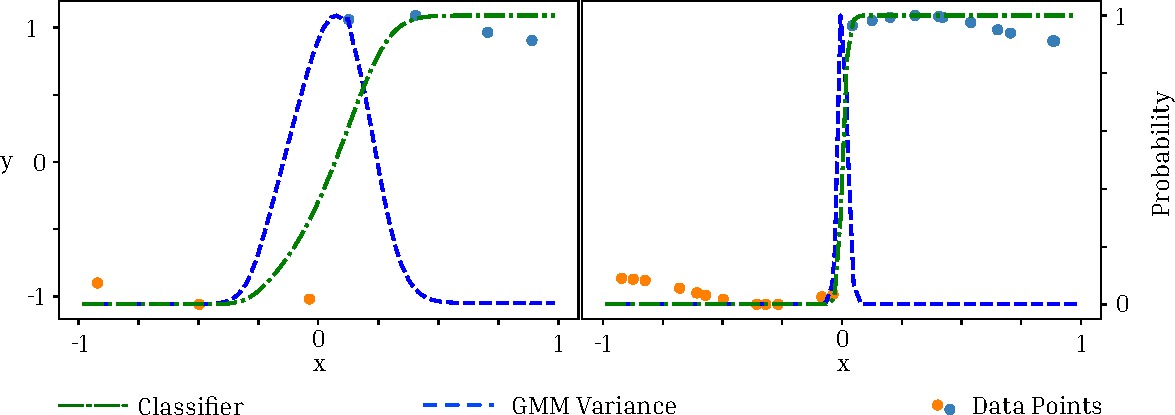
\includegraphics[width=\textwidth]{figures/sota_2/p_var.pdf}
    \caption{Schematic representation of the failure of variance-based \gls{al} strategies in the presence of a jump.}
    \label{fig:sota_2:active_learning}
\end{figure}

Fig.~\ref{fig:sota_2:active_learning} provides a schematic representation of the failure of variance-based \gls{al} strategies in the presence of a jump. Eq.~\eqref{eq:sota_2:mixture_var} is reported (normalized to be between 0 and 1) as a blue dashed line while the green line corresponds to the classifier probability $\mathbb{P}(\bx \in \Omega_1)$, which is close to 0 for $x < 0$ and close to 1 for $x > 0$. As we can see, adding points near the jump will never eliminate the model's uncertainty; the acquisition function spikes and the variance-based strategy would continuously select points near the jump.

\smallskip
The second case in which variance-based strategies fail is when we want to increase the training set size in batches. In this case, the second point must be discouraged from being selected near the first one, as it would not provide any new information. In \S\ref{sc:surr:select} we elegantly solved this last issue by performing a rank-1 update to the variance considering the \gls{evr}. In other words, we updated the variance of all candidate points by considering the effect of adding the first point to the training set (which only relies on the knowledge of its location and not its value).

\smallskip
Interestingly, considering the \gls{evr} elegantly solves also the first issue: in~\cite{cohn1996}, the authors propose to leverage the \gls{evr} to build an \gls{al} criterion, known as the \gls{alc} criterion, that samples the point that maximizes the expected reduction in variance over the entire input space. The \gls{alc} acquisition function is defined as:


\begin{equation}
    \alpha_{\text{ALC}}(\bx^\prime) = \int_{\Omega} \left( \mathbb{V}[\tilde{f}(\bx) \mid \data] - \mathbb{V}[\tilde{f}(\bx) \mid \data \cup \{\bx^\prime\}] \right) \mathbb{P}(\dd \bx) \;.
    \label{eq:conc:alc}
\end{equation}

The \gls{alc} criterion selects the point that mostly reduces the variance in the entire input space. Aside from actually selecting the point that yields the greatest uncertainty reduction, the \gls{alc} criterion discourages continuously choosing points near jumps as those have a high variance but are not informative for the global error. In practice, we replace the integral in Eq.~\eqref{eq:conc:alc} with a \gls{mc} estimate over a candidate set. 

\smallskip
The biggest limitation of Eq.~\eqref{eq:conc:alc} is that no closed-form expression for the \gls{evr} exists for a \gls{gmm} distribution. The main difficulty is that the distribution is not Gaussian, preventing us from efficiently computing rank-1 updates. This point requires future investigations. Notice that the \textit{soft reconstruction}, defined in Eq.~\eqref{eq:sota_2:soft_reconstruction}, is a Gaussian. Indeed, once the local \glspl{gp} and the classifier are trained, we can use their hyperparameters to define a new \gls{gp} prior, with mean and covariance defined as an average of the local covariances,

\begin{equation}
    \left.
        \begin{aligned}
            &m(\bx) = \summ{l}{1}{L} \mathbb{P}_{\mathrm{CLS}}(l \mid \bx, \boldsymbol{\gamma}) m_{\boldsymbol{\beta}_l}(\bx) \;,\\
            &k(\bx, \bx^\prime) = \summ{l}{1}{L} \mathbb{P}_{\mathrm{CLS}}(l \mid \bx, \boldsymbol{\gamma}) \mathbb{P}_{\mathrm{CLS}}(l \mid \bx^\prime, \boldsymbol{\gamma}) k_{\boldsymbol{\beta}_l}(\bx, \bx^\prime) \;.
        \end{aligned}
    \right.
    \label{eq:conc:gprec}
\end{equation}

Eq.~\eqref{eq:conc:gprec} can be derived from Eq.~\eqref{eq:sota_2:soft_reconstruction}, considering the \gls{gp} priors instead of the posteriors. Notice that the mean function is an average of the local means and the covariance an average of the local covariances. The hyperparameters in Eq.~\eqref{eq:conc:gprec} are already fixed from the model-clustering phase hence the \gls{gp} in Eq.~\eqref{eq:conc:gprec} only requires conditioning. 

\smallskip
Combining Eq.~\eqref{eq:conc:gprec} with the formulas in \S\ref{sec:ntools:evr} yields a novel \gls{al} criterion that can be used in combination with our model-based clustering loop. Specifically, at each iteration of the infilling strategy we first recompute the model-based clustering (starting from a fresh initial condition to forget potential errors), construct a candidate set by sampling from $\mathbb{P}(\dd x)$, and then compute the \gls{evr} of each candidate point using Eq.~\eqref{eq:conc:gprec} over the candidate set. The batch selection provides new points at which the function can be evaluated and added to the training set. 

\smallskip
In our tests, we did not see significant improvement (over variance-based strategies) that could justify the increase in computational cost. Yet, future research can investigate efficient ways to compute the \gls{evr} for a non-Gaussian mixture, improve the algorithmic implementation, and investigate how it scales as the dimension of the input space increases. Finally, an application combining such an \gls{al} strategy and calibration could constitute significant progress in the field.

\subsection{The Future of Uncertainty Quantification in in-Flight Icing Research}

The applications of \gls{uq} in the field of in-flight icing research are still in their infancy, although significant progress has been made in recent years. The main challenge is that the ice accretion process is, to the best of our knowledge, not fully understood, and models need to account for a variety of physical phenomena. A promising research direction is to move away from deterministic icing models and towards probabilistic models, such as the \textit{morphogenetic}~\cite{bellosta2024multi}, which combines a non-uniform droplet size injection with a stochastic ice-accretion approach based on the freezing probability of the water droplets. Morphogenetic approaches partially account for the uncertainty in the ice accretion process, and we firmly believe that they can be extended to account for a broader range of uncertainties. Combining such models with a robust uncertainty propagation of Appendix-C and Appendix-O conditions~\cite{Bellosta2021} could result in a much more faithful representation of the ice accretion process. 

\smallskip
A second research direction is to investigate the use of \gls{uq} techniques to better understand which parameters of the ice accretion process most significantly influence performance. Ice shapes, although being a standard output of computer codes and experimental measurements, are not repeatable, and we do not fully understand which geometrical parameters more strongly influence the performance. A major leap forward in this direction was achieved by~\cite{isi}, which introduced the \gls{isi}, a measure of the impact of ice accretion on the flying qualities of aircraft and drones. The \gls{isi} is a promising tool since it directly looks at the power-velocity curve, separating the effect of ice accretion into a mass effect (which adds weight to the aircraft) and a performance effect (which changes the aerodynamic properties of the aircraft). The \gls{isi} is a promising tool to investigate which parameters of the ice accretion process most strongly impact performance, and we believe that it can be used in combination with \gls{uq} techniques to better understand the ice accretion process. A second breakthrough could be achieved by combining such results with the work of~\cite{donizetti2026geometrical} which introduced geometrical similarity measures of ice shapes, and could be used to investigate how stochastic ice shapes and experimental ice shapes can be clustered together.

\smallskip
Finally, a third envisioned research direction is to investigate the use of \gls{uq} techniques in the context of robust design of aircraft anti-icing or de-icing systems. The design of such systems requires a choice of materials, geometries, and control strategies that can withstand a variety of operating conditions. In particular, the work of~\cite{GoriGallia2024} performed an optimization of the heat flux distribution of a thermal anti-icing system and showed that the optimal solution is very sensitive to the operating conditions, ultimately justifying the need for a robust design that could withstand a range of operating conditions. We believe that the use of such techniques can immediately provide measurable improvements in the current design of aircraft anti-icing or de-icing systems, and we envision that the next generation of such systems will be designed with \gls{uq} techniques in mind.